\chapter{SheepOS的功能实现}

SheepOS实现了若干比较简单的实验性功能,包括屏幕输出、中断、进程管理、
文件系统和若干小命令。

\section{简单的屏幕输出}

在之前没有\texttt{Print}函数,想在屏幕上输出文本时,不是利用BIOS中断就是利用系统调用,很
不方便,所以就需要为SheepOS增加属于它自己的\texttt{Print}函数。要实现一个\texttt{Print}函数大致可以
分为以下几个步骤(具体代码参见附录\ref{fsec:put_char}):

\begin{enumerate}
\item 备份寄存器;
\item 获取光标当前所处的位置坐标,该位置就是下一个可打印字符的位置;
\item 获取需要打印的字符;
\item 判断字符类型;如回车、换行、退格则会被特殊处理,除此之外将会直接输出显示;
\item 判断需不需要滚屏;
\item 更新光标的位置坐标,让它指向下一个打印字符的位置;
\item 恢复寄存器。
\end{enumerate}
这样就可以实现对单个字符的打印,效果如图\ref{fig:print_char}所示,这里只实现了对单个字符的
print,目前该效果是由多个\texttt{put\_char}来打印字符拼到一起来实现的。

\begin{figure}[H]
  \centering
  \includegraphics[width=.6\linewidth]{图3-8}
  \caption{字符打印}
  \label{fig:print_char}
\end{figure}

\begin{codeblock}
\begin{ccode}
int main(void)
{
    put_char('k');
    put_char('e');
    put_char('r');
    put_char('n');
    put_char('e');
    put_char('l');
    put_char('\n');
    put_char('1');
    put_char('2');
    put_char('\b');
    put_char('3');
    while(1);
}
\end{ccode}
\end{codeblock}

这样就形成了图\ref{fig:print_char}中的效果,在字符“kernel”最后换行符\verb|"\n"|也起到了效果,
成功换了行,而最后的“1”和“3”便是2和3之间的退格键\verb|"\b"|将字符“2”删除了,所以只留下了“1”和“3”。

\subsection{字符串的打印}
\label{subsec:str}

对于字符串Str的打印其实就是对单个字符打印函数进行一个封装。
方法如下:
\begin{itemize}
\item 声明全局函数
\begin{nasmcode}
global put_str
\end{nasmcode}
\item 备份ebx和ecx寄存器
\begin{nasmcode}
   push ebx
   push ecx
   xor ecx, ecx		      ; 准备用ecx存储参数,清空
   mov ebx, [esp + 12]	      ; 从栈中得到待打印的字符串地址 
.goon:
   mov cl, [ebx]
   cmp cl, 0		      ; 如果处理到了字符串尾,跳到结束处返回
   jz .str_over
   push ecx		      ; 为put_char函数传递参数
   call put_char
   add esp, 4		      ; 回收参数所占的栈空间
   inc ebx		      ; 使ebx指向下一个字符
   jmp .goon
.str_over:
   pop ecx
   pop ebx
   ret
\end{nasmcode}
\end{itemize}
% \iffalse
% \begin{nasmcode}
% global put_str
% put_str:
% ;由于本函数中只用到了ebx和ecx,只备份这两个寄存器
%    push ebx
%    push ecx
%    xor ecx, ecx		      ; 准备用ecx存储参数,清空
%    mov ebx, [esp + 12]	      ; 从栈中得到待打印的字符串地址 
% .goon:
%    mov cl, [ebx]
%    cmp cl, 0		      ; 如果处理到了字符串尾,跳到结束处返回
%    jz .str_over
%    push ecx		      ; 为put_char函数传递参数
%    call put_char
%    add esp, 4		      ; 回收参数所占的栈空间
%    inc ebx		      ; 使ebx指向下一个字符
%    jmp .goon
% .str_over:
%    pop ecx
%    pop ebx
%    ret
% \end{nasmcode}
% \fi
在有了\texttt{put\_char}之后\texttt{put\_str}无非就是多调用几个\texttt{put\_char}来进行打印最终达到字
符串的效果,只不过封装以后打印字符串就不用像之前那么繁琐,使用很多行代码来实现。效果如图\ref{fig:print_str}:

\begin{figure}[H]
  \centering
  \includegraphics[width=12cm]{图3-9}
  \caption{打印字符串}
  \label{fig:print_str}
\end{figure}

至此,SheepOS就可以在打印出来想要打印的东西。在有了\texttt{put\_str}之后打印这些字符就变得容易了许多:

\begin{codeblock}
\begin{ccode}
void main(void)
{
   put_str("I am str!\n");
   put_str("20211159013 CynYang\n");
   put_str("this is my OS!\n");
   while(1);
}
\end{ccode}  
\end{codeblock}

\subsection{整数的打印}
\label{subsec:int}
既然SheepOS有了能够打印Str的功能,那怎么能没有数字打印呢,在此次设计中只实现了对数字的打印,
原理就是将数字9转变为字符的'9'来输出,提到这个转换就不难想到ASCII码,
在ASCII码表中,字符0 \char`~\, 9的范围是48 \char`~\, 57,大写字母
A \char`~\, Z的范围是65 \char`~\, 90,所以
\begin{itemize}
\item 对数字的处理就是:0 \char`~\, 9之间的数字,用该数字加上字符'0'的ASCII码48;
\item 对字母的处理就是:A \char`~\, F之间的数字,用该数字减去10后再加上字符'A'的ASCII码65;
\end{itemize}
代码详见附录\ref{fsec:put_int}。
现在SheepOS就有一个简单的打印整形数的功能了。

\begin{ccode}
void main(void)
{
   put_str("I am Str\n");
   put_str("20211159013 CynYang\n");
   put_int(0);
   put_char('\n');
   put_int(9);
   put_char('\n');
   put_int(0x00021a3f);
   put_char('\n');
   put_int(0x12345678);
   put_char('\n');
   put_int(2023-04-03);
   while(1);
}
\end{ccode}

\begin{figure}[H]
  \centering
  \includegraphics[width=12cm]{图3-10}
  \caption{打印整形字符int}
  \label{fig:print_int}
\end{figure}
如图\ref{fig:print_int}所示。
它将输入的数字经过ASCII码表转换成对应的字符成功输出了。

\section{中断}
\label{sec:interrupt}

现在操作系统一直在做一件事情,那就是
\begin{codeblock}
\begin{ccode}
while(1)
{
  操作系统代码();
}
\end{ccode}  
\end{codeblock}
不论在其中完成了多少功能,它都是在进行一个死循环,要是没有中断的话,都不能使操作系统一边
处理图片,一边敲键盘聊天。就好似我正在玩一个游戏,但现在得跟朋友出去吃饭或是门铃响了要去开
门,若是没有暂停功能的话应该很难马上放开这个游戏去做别的事吧。操作系统的中断亦是如此,
正是因为有了中断,我们才能够同时享受计算机的多种服务。中断又分为两种:
\begin{itemize}
\item 外部中断:外部中断顾名思义就是CPU外部的中断,所以又叫做硬件中断。这个中断信号都是来自外部硬件的,如
网卡、磁盘控制器、键盘、鼠标、音频等等,与内部中断不同,它是异步的,就算有正在运行的指令,
它也能够发生。
\item 内部中断:又称为软中断,它通常作为CPU的异常处理,中断存在的意义主要是为了让计算机能够
  实现多任务,包括用户程序之间的切换、软件与软件之间的并存都需要有中断才能实现。
\end{itemize}

\subsection{中断描述符表}

中断描述符表就是保护模式下用于存储中断处理程序入口的表,当CPU收到一个中
断后,需要用中断向量在此表中检索对应的描述符,然后在描述符中找到中断处
理程序的起始地址,之后执行中断处理程序。如表\ref{tbl:idt}所示
\footnote{来源:\url{https://en.wikipedia.org/wiki/Interrupt_descriptor_table}},第一
列\texttt{INT\_NUM}表示中断向量号,共有255个,中断的机制就是在收到一个
中断信号后,调用相对应的中断处理程序,所以CPU在收到中断信号后,会根据中
断向量号去到中断描述符表中找到相应的中断程序的地址。

\begin{table}[!ht]
  \centering  \caption{中断描述符表\label{tbl:idt}}
  \begin{tblr}{width=\textwidth,colspec={rX[l]rX[l]},hline{1,2,Z}}
INT\_NUM & Short Description           & INT\_NUM & Short Description             \\
0x00     & Division by zero            & 0x0B     & Segment not present           \\           
0x01     & Single-step interrupt       & 0x0C     & Stack Segment Fault           \\           
0x02     & NMI                         & 0x0D     & General Protection Fault      \\      
0x03     & Breakpoint                  & 0x0E     & Page Fault \\                    
0x04     & Overflow                    & 0x0F     & reserved \\                      
0x05     & Bound Range Exceeded        & 0x10     & x87 Floating Point Exception  \\  
0x06     & Invalid Opcode              & 0x11     & Alignment Check \\               
0x07     & Coprocessor not available   & 0x12     & Machine Check \\                 
0x08     & Double Fault                & 0x13     & SIMD Floating-Point Exception \\ 
0x09     & Coprocessor Segment Overrun & 0x14     & Virtualization Exception      \\      
0x0A     & Invalid Task State Segment  & 0x15     & Control Protection Exception  \\
  \end{tblr}
\end{table}

\subsection{中断控制器8259A}

在认识中断的概念后,才知道操作系统真是太忙了,计算机上若是插入一个鼠标,操作系统要加
载一下,插入一个键盘,操作系统也要加载一下,本来操作系统就有很多自己的事情需要做了,所以就
需要一个部件来对这些中断进行统一的管理,而这个部件就是可编程中断控制器\texttt{8259A}。
\texttt{8259A}的作用是负责所有来自外设的中断,且它是可编程的,应该可以把它称作是打开中断的入口。
计算机内有两片\texttt{8259A}芯片,分别是主片和从片,如图\ref{fig:8259A}。

\begin{figure}[H]
  \centering
  \includegraphics[width=12cm]{图3-13}
  \caption{8259A芯片}
  \label{fig:8259A}
\end{figure}

\texttt{8259A}的芯片是直接安装在主板上的,所以可以直接对其进行操作,例如移动了一下鼠标,如图
\ref{fig:8259A}在\texttt{8259A}的从片\texttt{IRQ12}引脚处就会收到一个高电频,之后从片就会把该信息通过\texttt{8259A}主
片的\texttt{IRQ2}引脚传递到主片上,再从主片直接反映到CPU上说鼠标将要移动了请求CPU来处理。
那么处理其它中断也是一样的,在\texttt{8259A}收到一个优先级为多少的
中断后会告诉CPU:这是优先级靠前或是靠后的中断,需要进行处理。如图\ref{fig:interrupt_a}
在CPU收到后会根据中断向量号在中断描述符表中进行索引然后找出相应的选择子和偏移地址,在得到
选择子与偏移地址后,再到GDT中去寻找对应的描述段,之后就再在内存中找到该描述段的代码然后再
去执行。
进入中断的方法就是Kernel上调用中断处理函数,代码详见附录\ref{app:int_a}和\ref{app:int_b},
其过程如下:

\begin{itemize}
\item 如果是从片上进入的中断,除了往从片上发送\texttt{EOI}外,还要往主片上发送\texttt{EOI};
\item 调用\texttt{idt\_table}中的C版本中断处理函数;
\item 存储各个中断入口程序的地址,形成\texttt{intr\_entry\_table}数组
\end{itemize}

\begin{figure}[H]
  \centering
  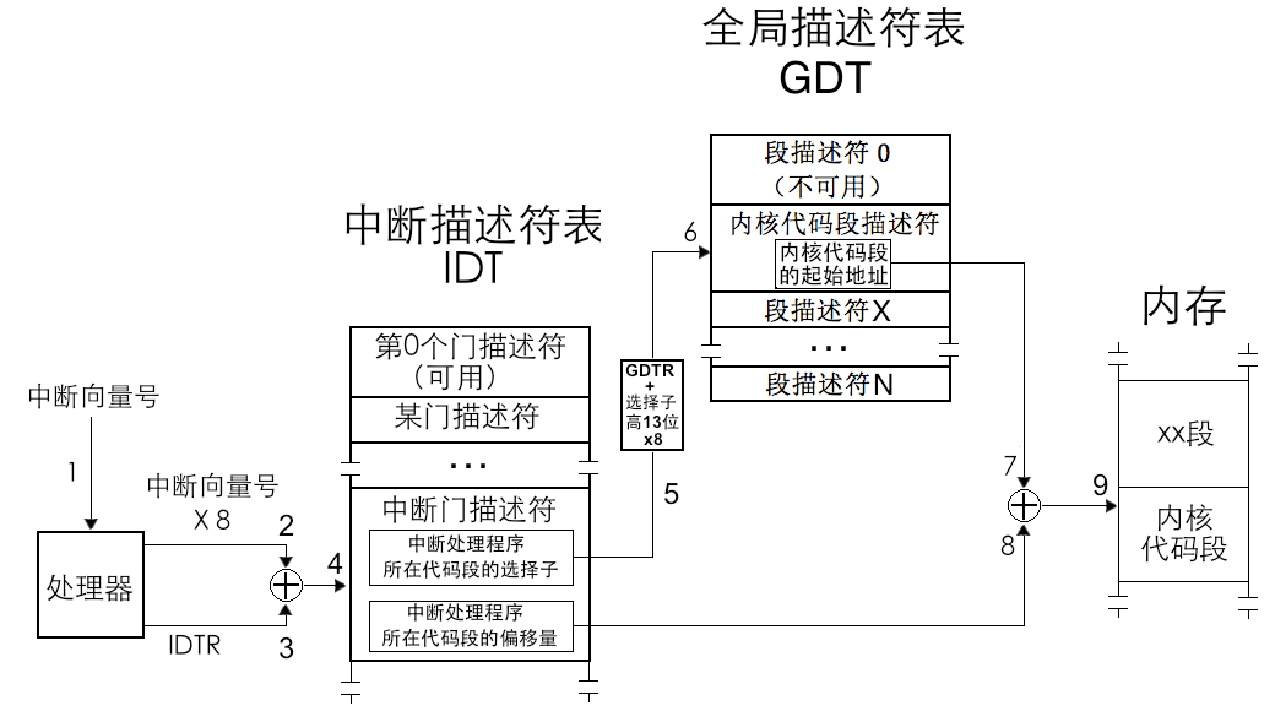
\includegraphics[width=.8\linewidth]{int-a}
  \caption{中断过程}
  \label{fig:interrupt_a}
\end{figure}

如图\ref{fig:8259A}所示,当向主片\texttt{0xA0}地址和从片\texttt{0x20}地址发送\texttt{EOI}后,就代表告诉\texttt{8259A}中断程序处理
结束了。

在进入中断前,还需要先保存中断发生前上下文的环境,以免发生数据丢失的情况,这里使用\texttt{PUSHAD}指
令压栈压入32位寄存器:
\begin{codeblock}
\begin{nasmcode}
   push ds
   push es
   push fs
   push gs
   pushad
\end{nasmcode}  
\end{codeblock}

在中断调用完后也需要用\texttt{POPAD}来恢复之前的环境:
\begin{codeblock}
\begin{nasmcode}
add esp, 4    ; 跳过中断号
   popad
   pop gs
   pop fs
   pop es
   pop ds
   add esp, 4 ; 跳过error_code
   iretd
\end{nasmcode}  
\end{codeblock}

至此就是\texttt{8259A}控制器的相关中断内容。

\subsection{键盘输入}

SheepOS现在已经有了中断,而在之前的图\ref{fig:8259A}上不难发现\texttt{8259A}主片\texttt{IRQ1}引脚对应
的是键盘,所以可以大胆试想一下,是不是SheepOS即将可以用键盘直接在屏幕上进行输入了?
答案是肯定的。

在此之前,首先简单介绍下键盘敲击的过程。在键盘中有着一个名为“键盘编译器”的芯片,它通常
是\texttt{8048}以及兼容芯片,作用就是监控键盘的输入,然后把数据发送给计算机,当然计算机主板上也有一
个键盘控制器,专门接受和解码来自键盘的数据,然后跟\texttt{8259A}和各个软件之间进行通信。敲击键盘的
步骤可以分为三种情况:
\begin{itemize}
\item 按下
\item 保持按下的状态
\item 松开
\end{itemize}
键盘按下松开后产生的编码叫做“扫描码”,当键盘按下和保持按下的时候产生\texttt{Make Code},而当松开
后会产生\texttt{Break Code}。在知道有扫描码的概念之后,就可以对照着键盘扫描码的
编码来与相应的字符进行处理。如附录\ref{sec:keyb}中的代码就是对键盘各个按键进行解析,之后就能
将字符正确的打印在屏幕上。如图\ref{fig:keybd},SheepOS现在就可以自由的在屏幕上输入任何想输入
的字符了。
\begin{figure}[H]
  \centering
  \includegraphics[width=15cm]{图3-14}
  \caption{键盘输入}
  \label{fig:keybd}
\end{figure}

\section{进程的实现}
\label{sec:course}
特权级的概念在前面图\ref{fig:tequan}中稍有提及,到现在SheepOS的程序一直是在最高特权级0级下运行
的,这非常危险,意味着用户程序有着跟操作系统同等的权限,想干什么干什么,若是有什么不听话的
程序的话,后果往往是灾难性的。操作系统存在的目的之一就是要管理资源的,所以操作系统可以一直
处于最高特权级,拥有最高的权利,但被管理的程序当然不能跟操作系统拥有同等的权利,所谓“一山
不容二虎”,一般情况下用户程序得处于特权级3级才行,所以在实现进程之前得先把权限的高低分清楚。

\subsection{从特权级0到特权级3}

一般情况下CPU是不允许从高特权级跳向低特权级的,所以如果想从特权级0跳到
特权级3的话,得采取一些手段,可以用从调用门和中断返回的手段来实现特权
级0->特权级3的转变,在SheepOS里使用的是中断返回的方式。既然要用中断返回,
那就少不了\texttt{iretd}指令\cite{ws2013},\texttt{iretd}指令会将栈中的
数据当作返回的地址,还会加载栈里的\texttt{eflags}的值到EFLAGS寄存器中,
若栈里的\texttt{cs.rpl}特权级更低的话,CPU的特权级Check通过后,还会
把\texttt{cs}载入到CS寄存器中,\texttt{ss}载入到SS寄存器中,之后CPU进入
低特权级。因此就必须在栈中的时候提前把数据准备妥当为\texttt{iretd}指令
使用。简单的说就是把进程前后的内容都存到栈里,然后通过\texttt{pop}把用
户进程的数据加载到寄存器,最后使用\texttt{iretd}退出中断。
\begin{itemize}
\item 退出中断的出口:\texttt{intr\_exit}函数;
\begin{codeblock}
\begin{nasmcode}
intr_exit:	     
; 以下是恢复上下文环境
   add esp, 4 ; 跳过中断号
   popad
   pop gs
   pop fs
   pop es
   pop ds
   add esp, 4 ; 跳过error_code
   iretd
\end{nasmcode}  
\end{codeblock}
\end{itemize}

该函数的作用是用来恢复发生中断时,被中断了的前后任务
状态,并且退出中断。在有了这些基础之后,只需将栈中存储的CS选择子里的RPL的值设为3,然后栈中
的段寄存器的选择子要指向DPL为3的内存段,使栈中\texttt{eflags}的\texttt{IF}位为1、
\texttt{IOPL}位为0,这样用户程序的
特权级就成为最低的第3位了。代码如下:
\begin{ccode}
void start_process(void* filename_)
{
   void* function = filename_;
   struct task_struct* cur = running_thread();
   cur->self_kstack += sizeof(struct thread_stack);
   struct intr_stack* proc_stack = (struct intr_stack*)cur->self_kstack;	 
   proc_stack->edi = proc_stack->esi = proc_stack->ebp = proc_stack->esp_dummy = 0;
   proc_stack->ebx = proc_stack->edx = proc_stack->ecx = proc_stack->eax = 0;
   proc_stack->gs = 0;		 // 用户态用不上,直接初始为0
   proc_stack->ds = proc_stack->es = proc_stack->fs = SELECTOR_U_DATA;
   proc_stack->eip = function;	 // 待执行的用户程序地址
   proc_stack->cs = SELECTOR_U_CODE;
   proc_stack->eflags = (EFLAGS_IOPL_0 | EFLAGS_MBS | EFLAGS_IF_1);
   proc_stack->esp = (void*)((uint32_t)get_a_page(PF_USER, USER_STACK3_VADDR) + PG_SIZE) ;
   proc_stack->ss = SELECTOR_U_DATA; 
   asm volatile ("movl %0, %%esp; jmp intr_exit" : : "g" (proc_stack) : "memory");
 }
\end{ccode}
用户进程的前后数据会保存在\texttt{struct intr\_stack}栈中,那么相同的\texttt{struck thread\_stack}就是用来保
存在中断处理程序的时候,切换任务时的前后文数据,其余是为8个通用寄存器进行初始化,在程序开
始运行之前,都没什么实际意义的值,因此直接初始化为0就行。

\subsection{创建用户进程}
创建用户进场的大概流程是:
\begin{itemize}
\item 先在内核中分配一页内存,为线程\texttt{thread}分配一页PCB\footnote{PCB(Process
    Control Block,进程控制块)是一种数据结构,用于存储和管理进程的状态信息。每个进程对应
    一个PCB,它包含着操作系统所需要的所有信息,以便操作系统对进程进行调度和管理。};
\item 初始化线程,为进程创建虚拟地址位图;
\item 创造一个为了调用初始化函数\texttt{start\_process}的线程;
\item 分配进程的页表空间;
\item 将带有初始化函数\texttt{start\_process}的线程放到就绪队列中,等待调用;
\end{itemize}

用户进程的详细代码在附录\ref{sec:process}中,大部分是页表项和页目录项的创建,因为为了方便操作
系统为用户进程提供各种系统功能的调用,就必须确保用户程序要在自己的地址空间中访问到内核才行,
也就是说内核空间得是用户空间的一部分,要做到这点的话,虚拟地址空间就得由页表控制,页表由操
作系统来管理,因此,用户进程的虚拟空间是由操作系统来进行规划和分配的。既然用户空间得由页表
来表示的话,那么就得用设置页表来解决了,所以创建用户进程的意义实质上就是为其创建页表。

\subsection{进程调度}
至此,用户进程已经创建完毕,并且已经准备就绪随时等待调用。进程调度
代码详见附录\ref{fsec:schedule}。调用的过程大致如下:
\begin{itemize}
\item 调用时钟中断处理函数;
\item 调用调度器函数\texttt{schedule};
\item 调用任务切换函数\texttt{switch\_to}.
\end{itemize}
对于进程的优先级高低,是通过调度器函数\texttt{schedule}中的\texttt{ticks}来衡量的,操作系
统会先给进程初始化一个优先级,再通过调用系统调用函数\texttt{get\_pid}调用查看进程执行的
ticks,再和初始化的优先级进行比对,最后根据最终的优先级对进程进行调度。

\section{文件系统}
\label{sec:file}

现在在SheepOS上虽然可以随意的敲击键盘输入字符,但这些字符始终都只是存在于屏幕上的东西,没
有任何的实际意义,而文件系统就是为了使这些东西拥有“生命”而存在的,让它们真真实实的存在于操作系统中。
对于LinuxOS而言,文件是最熟悉的东西了,在LinuxOS中的所有操作,可以说都是对文件进行操
作,包括使用的一些命令、脚本、甚至视频和图片,都是文件。

在创建文件系统之前,需要先定义三个数据结构。
\begin{itemize}
\item 超级块:
\begin{ccode}
struct super_block {
   uint32_t magic;		    // 用来标识文件系统类型,支持多文件系统的操作系统通过此标志来识别文件系统类型
   uint32_t sec_cnt;		    // 本分区总共的扇区数
   uint32_t inode_cnt;		    // 本分区中inode数量
   uint32_t part_lba_base;	    // 本分区的起始lba地址

   uint32_t block_bitmap_lba;	    // 块位图本身起始扇区地址
   uint32_t block_bitmap_sects;     // 扇区位图本身占用的扇区数量

   uint32_t inode_bitmap_lba;	    // i结点位图起始扇区lba地址
   uint32_t inode_bitmap_sects;	    // i结点位图占用的扇区数量

   uint32_t inode_table_lba;	    // i结点表起始扇区lba地址
   uint32_t inode_table_sects;	    // i结点表占用的扇区数量

   uint32_t data_start_lba;	    // 数据区开始的第一个扇区号
   uint32_t root_inode_no;	    // 根目录所在的I结点号
   uint32_t dir_entry_size;	    // 目录项大小

   uint8_t  pad[460];		    // 加上460字节,凑够512字节1扇区大小
} __attribute__ ((packed));
\end{ccode}
这里的数据块大小用的与扇区大小一致,也就是说1扇区$=$1块,因为后续磁盘操作要以扇区为单位,
这个数据块其实要不了那么多,所以最后加上460字节凑够512字节正好为1扇区。
\item inode结点:
\begin{ccode}
void inode_init(uint32_t inode_no, struct inode* new_inode) {
   new_inode->i_no = inode_no;
   new_inode->i_size = 0;
   new_inode->i_open_cnts = 0;
   new_inode->write_deny = false;

   /* 初始化块索引数组i_sector */
   uint8_t sec_idx = 0;
   while (sec_idx < 13) {
   /* i_sectors[12]为一级间接块地址 */
      new_inode->i_sectors[sec_idx] = 0;
      sec_idx++;
   }
}
\end{ccode}
  
\item 目录项:
\begin{ccode}
#define MAX_FILE_NAME_LEN  16
/* 目录结构 */
struct dir {
   struct inode* inode;   
   uint32_t dir_pos;	  // 记录在目录内的偏移
   uint8_t dir_buf[512];  // 目录的数据缓存
};

/* 目录项结构 */
struct dir_entry {
   char filename[MAX_FILE_NAME_LEN];  // 普通文件或目录名称
   uint32_t i_no;		      // 普通文件或目录对应的inode编号
   enum file_types f_type;	      // 文件类型
};
\end{ccode}
因为文件名要存储目录项里,所以目录项的大小是固定的,因此文件的名字长度也得有个限定,代码中
使用
\begin{ccode}
#define MAX_FILE_NAME_LEN  16
\end{ccode}
将其最大长度定义到了16个字符。
\end{itemize}
完成这些工作后,就可以对文件系统\cite{zsn2022}进行创建了,代码参见附录
\ref{app:partitionformat},创建的方法如下:
\begin{itemize}
\item 根据分区的容量,计算各分区文件系统元信息所需要的位置和扇区数;
\item 往内存里创建超级块,把上一步计算的元信息数据写入超级块;
\item 把超级块写入到磁盘里;
\item 把元信息写入磁盘上对应的地方;
\end{itemize}
至此,SheepOS已经有了基础的一个文件系统,之后对文件的操作都将建立在这个系统之上。

\subsection{创建文件}
在有了文件系统之后,就可以对文件进行相应的处理了,如创建、打开、关闭、删除文件等操作。
创建文件的操作只需要再增加一个\texttt{file\_create}的函数即可,代码参
见附录\ref{app:filecreate},其工作过程如下:
\begin{itemize}
\item 创建文件,若成功则返回文件描述符,否则返回-1;
\item 从堆中为inode申请内存;
\item 同步内存数据到硬盘;
\end{itemize}
以上就是\texttt{file\_creat}函数的创建过程,在\texttt{main.c}中直接调用该函数即可实现对文件的创建。

\subsection{文件的打开和关闭}
有了文件之后当然就需要对文件进行打开和关闭的操作了,这两个步骤实现的方法也很简单,就是
一个\texttt{file\_open}和\texttt{file\_close}的函数。代码参见附录
\ref{app:fileopen},其工作过程如下:
\begin{itemize}
\item 打开编号为\texttt{inode\_no}的inode对应的文件,若成功则返回文件描述符,否则返回-1;
\item 打开或创建文件成功后,返回文件描述符,否则返回-1;
\item 关闭文件;
\item 将文件描述符转化为文件表的下标;
\item 关闭文件描述符\texttt{fd}指向的文件,成功返回0,否则返回-1.
\end{itemize}

之后也是直接在\texttt{main.c}中调用这两个函数就可以实现对文件的打开和关闭操作。

\subsection{文件的写入和读取}
写入和读取的代码都很类似,也是两个函数,\texttt{file\_write}和\texttt{file\_read},写入和读取都有3个参数,
分别是:1)文件File;2)数据缓冲区Buf;3)字节数Count;这三个参数。

函数\texttt{file\_write}和\texttt{file\_read}的功能分别是:
\begin{itemize}
\item \texttt{file\_write}:把Buf里的Count个字节写入File;
\begin{ccode}
uint32_t write(int32_t fd, const void* buf, uint32_t count)
{
   return _syscall3(SYS_WRITE, fd, buf, count);
}
\end{ccode}
\item \texttt{file\_read}:读取Count个字节写入Buf;
\begin{ccode}
int32_t read(int32_t fd, void* buf, uint32_t count)
{
   return _syscall3(SYS_READ, fd, buf, count);
}
\end{ccode}
\end{itemize}

\subsection{删除文件}

删除文件用的是\texttt{unlink}函数,而删除文件可以理解为与创建文件相反的一个过程,怎么创建的文件就怎
么删除,所以会涉及到inode、位图、目录项、目录inode中的
\texttt{i\_size}、数据块等数据的回收。代码详见附录\ref{app:filedel},工作过程如下:
\begin{itemize}
\item 回收inode;
\item 接下来是删除目录项;
\item 创建\texttt{sys\_unlink}函数。
\end{itemize}
至此,就完成了文件的删除操作。

\section{一个简单shell的实现}
\label{sec:shell}
现在SheepOS有了一套属于自己的文件系统,但是对这些文件进行操作的话还得在程序里通过调用之后
编译才能实现,操作系统本就是为用户服务的,所以用户和操作系统之间的交互尤为重要,
Shell的存在就是为了使用户与操作系统直接能够更直接的进行互动。Shell的功能大概就是能够收到用
户输入的指令,解析输入的字符是内部指令还是外部指令,然后执行与用户输入的指令相关的操作。
\begin{itemize}
\item 存储输入的命令:
\begin{ccode}
static char cmd_line[MAX_PATH_LEN] = {0};
char final_path[MAX_PATH_LEN] = {0};
\end{ccode}

\item 用来记录当前目录,是当前目录的缓存,每次执行\texttt{cd}命令时会更新此内容:
\begin{ccode}
char cwd_cache[MAX_PATH_LEN] = {0};
\end{ccode}

\item 输出提示符:
\begin{ccode}
void print_prompt(void)
{
   printf("[yx@SheepOS %s]$ ", cwd_cache);
}
\end{ccode}
\end{itemize}

Shell就像是为用户和操作系统之间搭了一把梯子,有了这个梯子之后用户有什么需求可以直接向操作
系统伸出手去索要,而操作系统也能直接把我们想要的东西递交到我们的手中。
接下来就向操作系统发出第一个需求:清屏和清除输入内容。

\begin{ccode}
void my_shell(void) {
   cwd_cache[0] = '/';
   while (1) {
      print_prompt(); 
      memset(final_path, 0, MAX_PATH_LEN);
      memset(cmd_line, 0, MAX_PATH_LEN);
      readline(cmd_line, MAX_PATH_LEN);
      if (cmd_line[0] == 0) {	 // 若只键入了一个回车
	 continue;
      }

      argc = -1;
      argc = cmd_parse(cmd_line, argv, ' ');
      if (argc == -1) {
	 printf("num of arguments exceed %d\n", MAX_ARG_NR);
	 continue;
      }
\end{ccode}

\subsection{\Ctrl{L} 和 \Ctrl{U}}

这两个组合键需要用到之前提到过的键盘扫描码,代码如下:

\begin{itemize}
\item 清屏\Ctrl{L}:
\begin{ccode}
	 case 'l' - 'a': 
	    /* 1 先将当前的字符'l'-'a'置为0 */
	    *pos = 0;
	    /* 2 再将屏幕清空 */
	    clear();
	    /* 3 打印提示符 */
	    print_prompt();
	    /* 4 将之前键入的内容再次打印 */
	    printf("%s", buf);
	    break;
\end{ccode}
  
\item 清除输入\Ctrl{U}:
\begin{ccode}
	 case 'u' - 'a':
	    while (buf != pos) {
	       putchar('\b');
	       *(pos--) = 0;
	    }
	    break;
\end{ccode}
\end{itemize}

繁杂的工作在之前就已经差不多做完了,所以在Shell中基本上只需要直接调用之前写好的函数就可以
。

\subsection{打印目录清单(ls)}
\begin{itemize}
\item 利用Shell的内部命令建立ls函数:
\begin{ccode}
      void buildin_ls(uint32_t argc, char** argv)
\end{ccode}
\item 检测符号"-",如果是则\texttt{ls}后视为参数(目前只支持\texttt{-h}和\texttt{-l}):
\begin{ccode}
      if (argv[arg_idx][0] == '-')
      {	
	 if (!strcmp("-l", argv[arg_idx])) {         // 如果是参数-l
	    long_info = true;
	 } else if (!strcmp("-h", argv[arg_idx])) {   // 参数-h
	    printf("usage: -l list all infomation about the file.\n-h for help\nlist all files in the current dirctory if no option\n"); 
	    return;
	 } else {	
	    printf("ls: invalid option %s\nTry `ls -h' for more information.\n", argv[arg_idx]);
	    return;
	 }
      }
\end{ccode}
\item 若\texttt{ls}后参数是\texttt{-l}的话则把\texttt{long\_info}置为true,可以理解为显示文件详细信息的开关:
\begin{ccode}
      if (long_info)
      {
	 printf("-  %d  %d  %s\n", file_stat.st_ino, file_stat.st_size, pathname);
      } else {
	 printf("%s\n", pathname);  
      }
\end{ccode}
\item 若\texttt{ls}后不是参数,则视为路径参数且只能为1个,超过做出提示:
\begin{ccode}
	 if (arg_path_nr == 0) {
	    pathname = argv[arg_idx];
	    arg_path_nr = 1;
	 } else {
	    printf("ls: only support one path\n");
	    return;
	 }
\end{ccode}
\item 如果只输入了\texttt{ls}或\texttt{ls -l}则默认以当前路径处理:
\begin{ccode}
   if (pathname == NULL)
   {	
      if (NULL != getcwd(final_path, MAX_PATH_LEN)) {
	 pathname = final_path;
      } else {
	 printf("ls: getcwd for default path failed\n");
	 return;
      }
   } else {
      make_clear_abs_path(pathname, final_path);
      pathname = final_path;
   }
\end{ccode}
\item 如果在目录中没有找到指定路径,则提示:
\begin{ccode}
   if (stat(pathname, &file_stat) == -1)
   {
      printf("ls: cannot access %s: No such file or directory\n", pathname);
      return;
   }
\end{ccode}
\end{itemize}

\subsection{跳转到指定目录(cd)}

\begin{itemize}
\item 利用shell的内部命令建立cd函数:
\begin{ccode}
   char* buildin_cd(uint32_t argc, char** argv)
\end{ccode}
\item 设定参数限制,若参数大于1个,则做出提示:
\begin{ccode}
   if (argc > 2)
   {
      printf("cd: only support 1 argument!\n");
      return NULL;
   }
\end{ccode}
\item 若只键入了\texttt{cd}而无参数的话,返回根目录:
\begin{ccode}
   if (argc == 1)
   {
      final_path[0] = '/';
      final_path[1] = 0;
   } else {
      make_clear_abs_path(argv[1], final_path);
   }
\end{ccode}
\item 如果没有找到指定的目录,则做出提示:
\begin{ccode}
   if (chdir(final_path) == -1)
   {
      printf("cd: no such directory %s\n", final_path);
      return NULL;
   }
\end{ccode}
\end{itemize}

\subsection{创建文件(mkdir)}

\begin{itemize}
\item 利用shell的内部命令建立\texttt{mkdir}函数:
\begin{ccode}
   int32_t buildin_mkdir(uint32_t argc, char** argv)
\end{ccode}

\item 设定参数限制,只能有一个参数就是文件名字:
\begin{ccode}
   if (argc != 2)
   {
      printf("mkdir: only support 1 argument!\n");
   }
\end{ccode}

\item 创建文件
\begin{ccode}
   make_clear_abs_path(argv[1], final_path);
     if (strcmp("/", final_path))
     {
       if (mkdir(final_path) == 0)
         {
	    ret = 0;
	 } else {
	    printf("mkdir: create directory %s failed.\n", argv[1]);
	 }
     }
   }
\end{ccode}
\end{itemize}

\texttt{argv[1]}表示要创建的文件名,\texttt{final\_path}是文件的路
径,\texttt{strcmp("/",final\_path)}用来判断创建的文件是否是在根目录
下。

\subsection{删除文件(rmdir)}

删除文件与创建文件代码基本相似,毕竟就是一个创建文件的逆过程。
\begin{itemize}
\item 利用shell的内部命令建立\texttt{rm}函数:
\begin{ccode}
   int32_t buildin_rm(uint32_t argc, char** argv)
\end{ccode}
删除和判断是否在根目录的方法与创建文件相同。
\item 调用\texttt{unlink}函数释放相应路径里的数据:
\begin{ccode}
   if (unlink(final_path) == 0)
   {
      ret = 0;
   } else {
     printf("rm: delete %s failed.\n", argv[1]);
   }
\end{ccode}
\end{itemize}
%%% Local Variables:
%%% mode: latex
%%% TeX-master: "../thesis"
%%% End:
